                                                                                                      \documentclass[main.tex]{subfiles}


\begin{document}
\chapter{Results and Discussion}


\begin{figure}[h!]
\centering
\begin{subfigure}[t]{0.75\textwidth}

\includestandalone[mode=image,build={quote={}}]{"pgfplots/C_P"}

\caption{Point load}
\label{fig:C_P}
\end{subfigure} \hfill
\begin{subfigure}[t]{0.24\textwidth}

\includestandalone[mode=image,build={quote={}}]{"tikz/Mesh_Density"}

\caption{Mesh}
\label{fig:Mesh_Density}
\end{subfigure}
\vfill
\vspace{1cm}

\begin{subfigure}[t]{0.75\textwidth}
\centering
\includestandalone[mode=image,build={quote={}}]{"pgfplots/C_q"}

\caption{Distributed load}
\label{fig:C_q}
\end{subfigure} \hfill
\begin{subfigure}[t]{0.24\textwidth}
\centering
\includestandalone[mode=image,build={quote={}}]{"tikz/Load_P_q"}

\caption{Loads}
\label{fig:Load_P_q}
\end{subfigure}
\vspace{1cm}
\caption{Convergence of elements on different loading and boundary conditions.}
\end{figure} \par

To effectively validate both the elements given in chapter.3, multiple convergence tests were studied. To study the effect of boundary conditions and loads, a circular plat with point load and distributed load is analysed for both elements. Here,  the element is simply supported on one side and fixed on other side. The same simulation is done for increasing mesh density (figure:  \ref{fig:Mesh_Density}). The simulation results are plotted in figure : \ref{fig:C_P}. Difference between analytical solution (equation :\ref{eq:C_P_SS},equation : \ref{eq:C_P_BI})(see.\cite{TIMOPLATES}) and numerical solution(figure.A.1 and figure.A.2) at the center of the circular plate where the displacement is maximum is considered as error. \par
Analytically solution of simply supported circular plate with point load.

\begin{equation}{\label{eq:C_P_SS}}
w=\frac{P}{16 \pi D} \left[\frac{3+\nu}{1+\nu}\left(a^2-r^2\right)+2r^2log\frac{r}{a}\right]
\end{equation}
\\
Analytically solution of build-in circular plate with point load.

\begin{equation}{\label{eq:C_P_BI}}
w=\frac{Pr^2}{8 \pi D} log\frac{r}{a}+\frac{P}{16 \pi D} \left(a^2 - r^2 \right)
\end{equation}\par
Where, r is the distance from the center of the circle. From the figure.\ref{fig:C_P}, It can be noted that both the elements converges faster for simply supporter boundary condition.For the application of hot dip galvanization, only simply supported boundary condition is necessary. So lack of fast convergence in build-in Boundary condition is not a concern. It can also be noted that the QUAD4 element preforms better than PAT element. Same analysis is also done where load is equally distributed on the surface. the analytically solution of the problem is given by equation.\ref{eq:C_q_SS} and equation.\ref{eq:C_q_BI} (see. \cite{TIMOPLATES}).
\\
\\
Analytical displacement at the center of simply supported circular plate with Distributed Load.

\begin{equation}{\label{eq:C_q_SS}}
w_{max}=\frac{\left(5+\nu\right)qa^4}{64 D \left(1+\nu\right)} 
\end{equation}
\\
Analytical displacement at the center of Build-in circular plate with Distributed Load.

\begin{equation}{\label{eq:C_q_BI}}
w_{max}=\frac{qa^4}{64 D} 
\end{equation}
\par
From the figure : \ref{fig:C_q}, the Point to notice is that the PAT element performs better for distributed load. Similar to the previous case. The FEM program doesn't converge fast for the build-in load. From this analysis, it can be stated that PAT element with simply supported boundary condition is a better option if distributed load is involved.  \par

The steel strip in hot dip galvaniwation is axially stressed, to understand the convergence of both elements during axial load, a modal analysis is performed where an axial stress of N is applied in the direction of y axis. The dominent natural frequency is computed and compared with the analytical natural frequency (equation . \ref{eq:S_N}) (\cite{LEISSA_NASA}). Corresponding mesh density and load description is given in figure . \ref{fig:Mesh_Density_S}. 

The natural frequency of a plate with membrane stress. 'a' is the length of the side.

\begin{equation}{\label{eq:S_N}}
\rho \omega_{mn}^{2} = D \left[ \left( \frac{\pi}{a}\right)^2 \right]^2 + N \left(\frac{\pi}{a} \right)^2 
\end{equation} 

\begin{figure}[t]
\centering
\begin{subfigure}[t]{0.75\textwidth}
\centering
\includestandalone[mode=image,build={quote={}}]{"pgfplots/S_N"}

\caption{Plot of error against mesh density}
\label{fig:S_N}
\end{subfigure} \hfill
\begin{subfigure}[t]{0.24\textwidth}
\centering
\includestandalone[mode=image,build={quote={}}]{"tikz/Mesh_Density_S"}

\caption{Mesh}
\label{fig:Mesh_Density_S}
\end{subfigure}

\caption{Convergence of natural frequency of square plate with axial load}
\end{figure}

The convergence of Natural frequency for a square plate with membrane load is given in the figure:\ref{fig:S_N}. It is clearly noted that the QUAD4 element converges much faster then than PAT element. One point to notice is that, the loads are applied such that the membrane-bending interaction stiffness contribution is very high such that it overshadows pure bending stiffness. Apparently this is the case for actual loading in hot dip galvanization application(figure.A.3). 

\begin{figure}[h!]
\centering
\includestandalone[mode=image,build={quote={}}]{"tikz/Strip_load_FvsD"}
\caption{Strip with imposed displacement and transverse load}
\label{fig:Strip_LOAD_FvsD1}
\end{figure}
\begin{figure}[h!]
\centering
\includestandalone[mode=image,build={quote={}}]{"tikz/Strip_Mesh_Density"}
\caption{Mesh density of strip}
\label{fig:Strip_Mesh_Density}
\end{figure}
\begin{figure}[h!]
\centering
\includestandalone[mode=image,build={quote={}}]{"pgfplots/Strip_FvsD_PAT"}
\caption{Comparision of solution between $w$ and $F$ for PAT element}
\label{fig:Strip_FvsD_PAT}
\end{figure}
\begin{figure}[h!]
\centering
\includestandalone[mode=image,build={quote={}}]{"pgfplots/Strip_FvsD_MITC4"}
\caption{Comparision of solution between $w$ and $F$ for QUAD4 element}
\label{fig:Strip_FvsD_MITC4}
\end{figure}

To study the behavior of the plate with imposed displacement and transverse forces,an analysis is done on a long metal strip of length 10m, width 1m figure. \ref{fig:Strip_LOAD_FvsD1}. The plate is simply supported on  one end and a sinusoidal displacement on other end and sinusoidal distributed load is applied on the middle of the plate. The figure. \ref{fig:Strip_Mesh_Density} shows the mesh of the strip with density of 2. Two Point P1 and P2 are used for measuring the results and error is calculated. 





PAT element is analyzed first. Imposed sinusoidal displacement of strip with increasing mesh density. The data is measured at two points P1 and P2. P1 is at the center of the strip and P2 is 2.5 m away from where the displacement is imposed(fig:A.4). Figure .  \ref{fig:Strip_FvsD_PAT} shows the result of the study. It evident that the result converges, but error is higher for small mesh density. It is noted that position of error also does not have huge impact. In same figure, the convergence of strip with transverse load is also plotted. It is clear that the transverse load has little to no effect on mesh density. 


When the QUAD4 element is provided with the sinusoidal boundary condition the solution takes longer to converge fig : \ref{fig:Strip_FvsD_MITC4}. But again, when the transverse load is applied it also has no effect on mesh density. From this analysis it clear that when there is imposed displacement at the boundaries the mesh density has to very fine but at the same time the mesh density has little effect of transverse load. 

\begin{figure}[h]
\centering
\includestandalone[mode=image,build={quote={}}]{"tikz/Mesh_Density_NbvsNl"}
\caption{Directional mesh density}
\label{fig:Mesh_Density_NbvsNl}
\end{figure}
\begin{figure}[h]
\centering
\includestandalone[mode=image,build={quote={}}]{"pgfplots/Strip_nlvsnb_nb"}
\caption{Comparison of elements with different directional mesh density in x direction}
\label{fig:Strip_nlvsnb_nb}
\end{figure}
\begin{figure}[h!]
\includestandalone[mode=image,build={quote={}}]{"pgfplots/Strip_nlvsnb_nl"}
\caption{Comparison of elements with different directional mesh density in y direction}
\label{fig:Strip_nlvsnb_nl}
\end{figure}

To understand the effect of directional mesh density, a study is done where the number of elements in one direction is increased consistently and in other direction is kept. This analysis also helped in understand the effect of mesh density to the direction in which material is moving. For the study, same strip is taken but the meshes are not prefect squares instead they are rectangles whose aspect ratio changes according to the given $nL$ and $nB$ values. $nL$ is the number of elements in on y direction similarly $nB$ is the number of elements in x direction(figure.\ref{fig:Mesh_Density_NbvsNl}). Figure. \ref{fig:Strip_nlvsnb_nb} shows the effect of direction density, if the mesh density is increased in direction perpendicular to material transport velocity. It is clear that the QUAD4 element is not affected. But the PAT element is affected by it, It may be because of the shape of the element. Figure . \ref{fig:Strip_nlvsnb_nl} shows the effect of results when the mesh density is increased in the parallel direction of line speed. It is evident from this analysis that the element size has to be very fine in the direction of material moving. 

\begin{figure}[h!]
\includestandalone[mode=image,build={quote={}}]{"pgfplots/Strip_SR"}
\caption{Comarison of PAT and MITC4 elements for different mesh density skewness}
\label{fig:Strip_SR}
\end{figure}

\begin{figure}[h]
\centering
\includestandalone[mode=image,build={quote={}}]{"tikz/Strip_load_MD"}
\caption{Mesh density skewness}
\label{fig:Strip_load_SR}
\end{figure}

From the previous study, it is clear that the mesh density in the direction of the axial velocity is very important. It is not clear whether the over all element size affect the result or the element size at the boundary at which the time dependent Dirichlet load in applied. Skewed Mesh density is applied on a strip to understand its effect (figure .\ref{fig:Strip_load_SR}). The solution converges as the mesh density reached 1.05 and it stay converged as the skewness ratio increases even though the element size at points P1 and P2 increases with large mesh density skewness \ref{fig:Strip_SR}. Which tell us that the element size has to be very small only on the boundary where the Dirichlet load is applied and also at the direction of the line speed. This idea is also enforced by the fact that the convergence rate between the points P1 and P2 is not vastly different. 

\begin{figure}[h!]
\centering
\includestandalone[width=\linewidth,mode=image,build={quote={}}]{"tikz/strip_mesh_zoom"}
\caption{Optimized FE mesh}
\label{fig:strip_mesh_zoom}
\end{figure}

\begin{figure}[h!]
\centering
\includestandalone[mode=image,build={quote={}}]{"pgfplots/FEMvsGal"}
\caption{Comparison of FEM with existing Galarkin method}
\label{fig:FEMvsGAL_Plot}
\end{figure}



%\begin{figure}[h!]
%\centering
%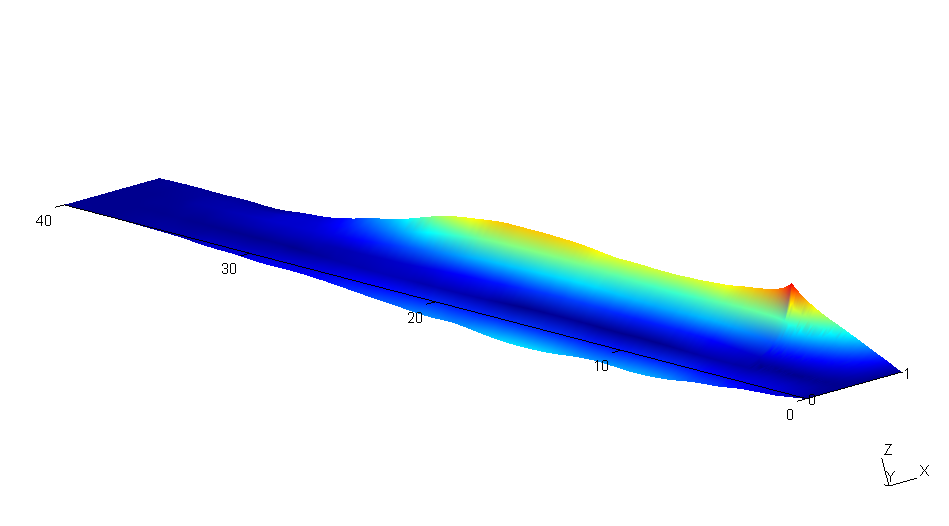
\includegraphics[width=\linewidth,trim={0 0 0 0},clip]{images/FEMvsGAL.png}
%\caption{Displcement plot of }
%\label{fig:FEMvsGAL_RES}
%\end{figure}

The Finite element program that is created during this thesis is compared with the existing Galerkin based numerical simulation tool. Result with QUAD4 element agrees with the solution of the Galerkin method figure.\ref{fig:FEMvsGAL_Plot}. But the FEM solution with PAT element has noticeable difference in the result. The solution is in the figure. A.5.


\begin{figure}[h!]
\centering
\includestandalone[mode=image,build={quote={}}]{"pgfplots/Strip_Para_V"}
\caption{A plate with different axial velocity}
\label{fig:Strip_Para_V}
\end{figure}

Strip with different line velocity is studied and the result are plotted in figure.\ref{fig:Strip_Para_V}. The solution agrees with the analytical solution calculated.


\end{document}
